\RequirePackage{luatex85}
\PassOptionsToPackage{shorthands=off}{babel}
\makeatletter
\disable@package@load{fontenc}
\makeatother
\let\oldlooseness=\looseness
\documentclass{csbulletin}
\selectlanguage{czech}
\setcounter{secnumdepth}{3}
\usepackage{titlesec}
\titlelabel{\thetitle\enspace}
\usepackage{luavlna}
\usepackage[strict]{lua-widow-control}
\usepackage{csquotes}
\usepackage[
  backend=biber,
  style=iso-numeric,
  sortlocale=cs,
  autolang=other,
  bibencoding=UTF8,
  mincitenames=2,
  maxcitenames=2,
  doi=false,
]{biblatex}
\renewcommand\multicitedelim{\addsemicolon\space}
\addbibresource{main.bib}
\usepackage[
  implicit=false,
  hidelinks,
]{hyperref}
\usepackage{hologo}
\usepackage{caption}

\newcommand\acro[1]{\textsc{\MakeLowercase{#1}}}
\newcommand\pkg{\textsf}

\ExplSyntaxOn
\newcommand
  \inputsubtitles
  [3]
  []
  {
    \sys_get_shell:nnN
      {
        sed~-r~-n~'/^#2$/,/^#3$/ {
          /^[0-9]+$/ ! {
            /..:..:..,...~-->~..:..:..,.../ ! {
              /./~
              {
                s/LaTeX2e/|LaTeXe{}/g;
                s/(^|~)LaTeX/~|LaTeX{}/g;
                s/>LaTeX/>|LaTeX{}/g;
                s/ConTeXt|XeTeX|LuaTeX|pdfTeX/|hologo{&}/g;
                s/OpTeX/Op|TeX{}/g;
                s/HTML|YAML|JSON|XML|CTAN/|acro{&}/g;
                s/tinyyaml|lt3luabridge/|pkg{&}/g;
                s/hardLineBreaks|.markinline/|texttt{&}/g;
                s/(^|~)TeX/~|TeX{}/g;
                s/>TeX/>|TeX{}/g;
                s/<i>[^<]*/|emph{&}/g;
                s/<[^>]*>//g;
                #1
                p
              }
            }
          }
        }'~markdown-3-cs.srt
      }
      {
        \char_set_catcode_other:N \\
        \char_set_catcode_other:N \%
        \char_set_catcode_escape:N |
      }
      \l_tmpa_tl
    \tl_trim_spaces:N
      \l_tmpa_tl
    \tl_use:N
      \l_tmpa_tl
  }
\ExplSyntaxOff
\begin{document}

\singlechars{czech}{AaIiVvOoUuSsZzKk}
\hyphenation{mark-down Mark-down mark-downu Mark-downu}

\title{Markdown 3: Co je nového a co se chystá?}
\EnglishTitle{Markdown 3: What's New, What's Next?}
\author{Vít Starý Novotný}
\podpis{Vít Starý Novotný, witiko@mail.muni.cz}
\maketitle[1ex]

\begin{abstract}
\oldlooseness=-1
\TeX ový balíček Markdown poskytuje posledních osm let rozšiřitelný a formátově agnostický značkovací jazyk. V článku představuji třetí verzi balíčku Markdown a změny, které přináší ve srovnání s verzí 2.10.0. Zaměřuji se na tři hlavní skupiny uživatelů balíčku Markdown. Spisovatelé se dozvědí o nových prvcích, které mohou používat ve svých dokumentech, \TeX perti se naučí určovat styl prvků jazyka markdown v různých formátech \TeX u a vývojáři nahlédnou pod pokličku správy a vývoje balíčku Markdown a naučí se přidávat podporu pro nové prvky jazyka markdown. Článek je překlad mé přednášky na TUGu 2023~\cite{novotny2023markdowna, novotny2023markdownb}.
% TODO: Článek je přeložený přepis mé přednášky na TUGu 2023 doplněný o fotografie, ukázky kódu a bibliografické odkazy.
\end{abstract}
\klicovaslova: Markdown, CommonMark, Lua, \TeX, \LaTeX, Op\TeX, Pandoc

\section{Úvod}
\inputsubtitles{1}{7}

% Motivace pro spisovatele, TeXperty a vývojáře
% Osnova článku
% Odkaz na [slajdy][1] a [videozáznam][2], fotografie/screenshot přednášky
%
% [1]: https://tug.org/tug2023/files/sa-03-novotny-markdown3/novotny-markdown3-slides.pdf
% [2]: https://youtu.be/U8XjTOhJkg0

\subsection{Motivace pro spisovatele}

\inputsubtitles{7}{8}

\inputsubtitles{8}{16}

\begin{figure}[t]
\fboxsep=0pt\relax
\textcolor{Gray}{\fbox{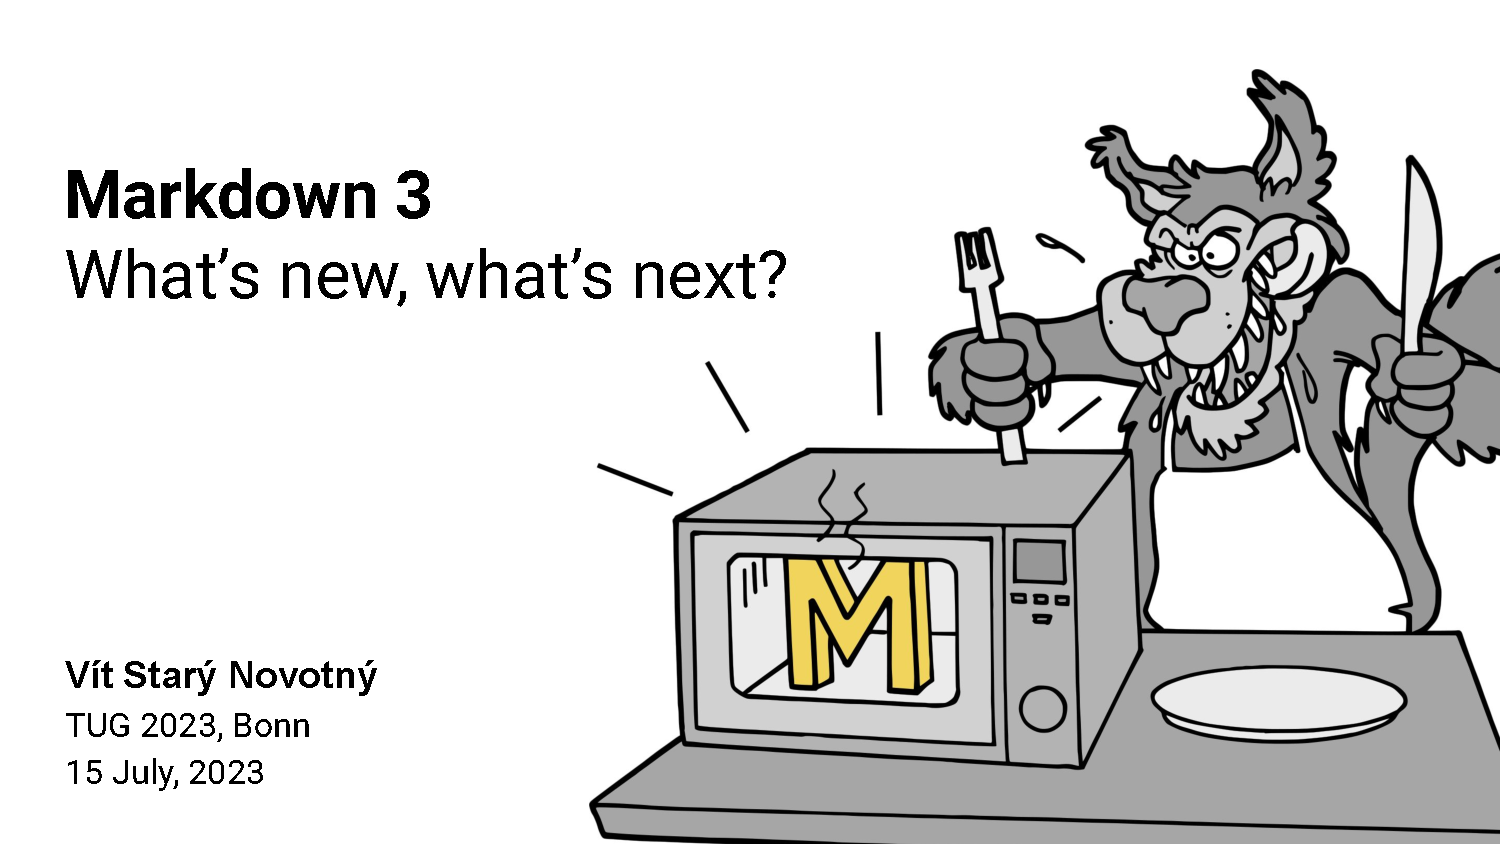
\includegraphics[width=0.55\linewidth]{figs/talk-background}}}%
\hfill
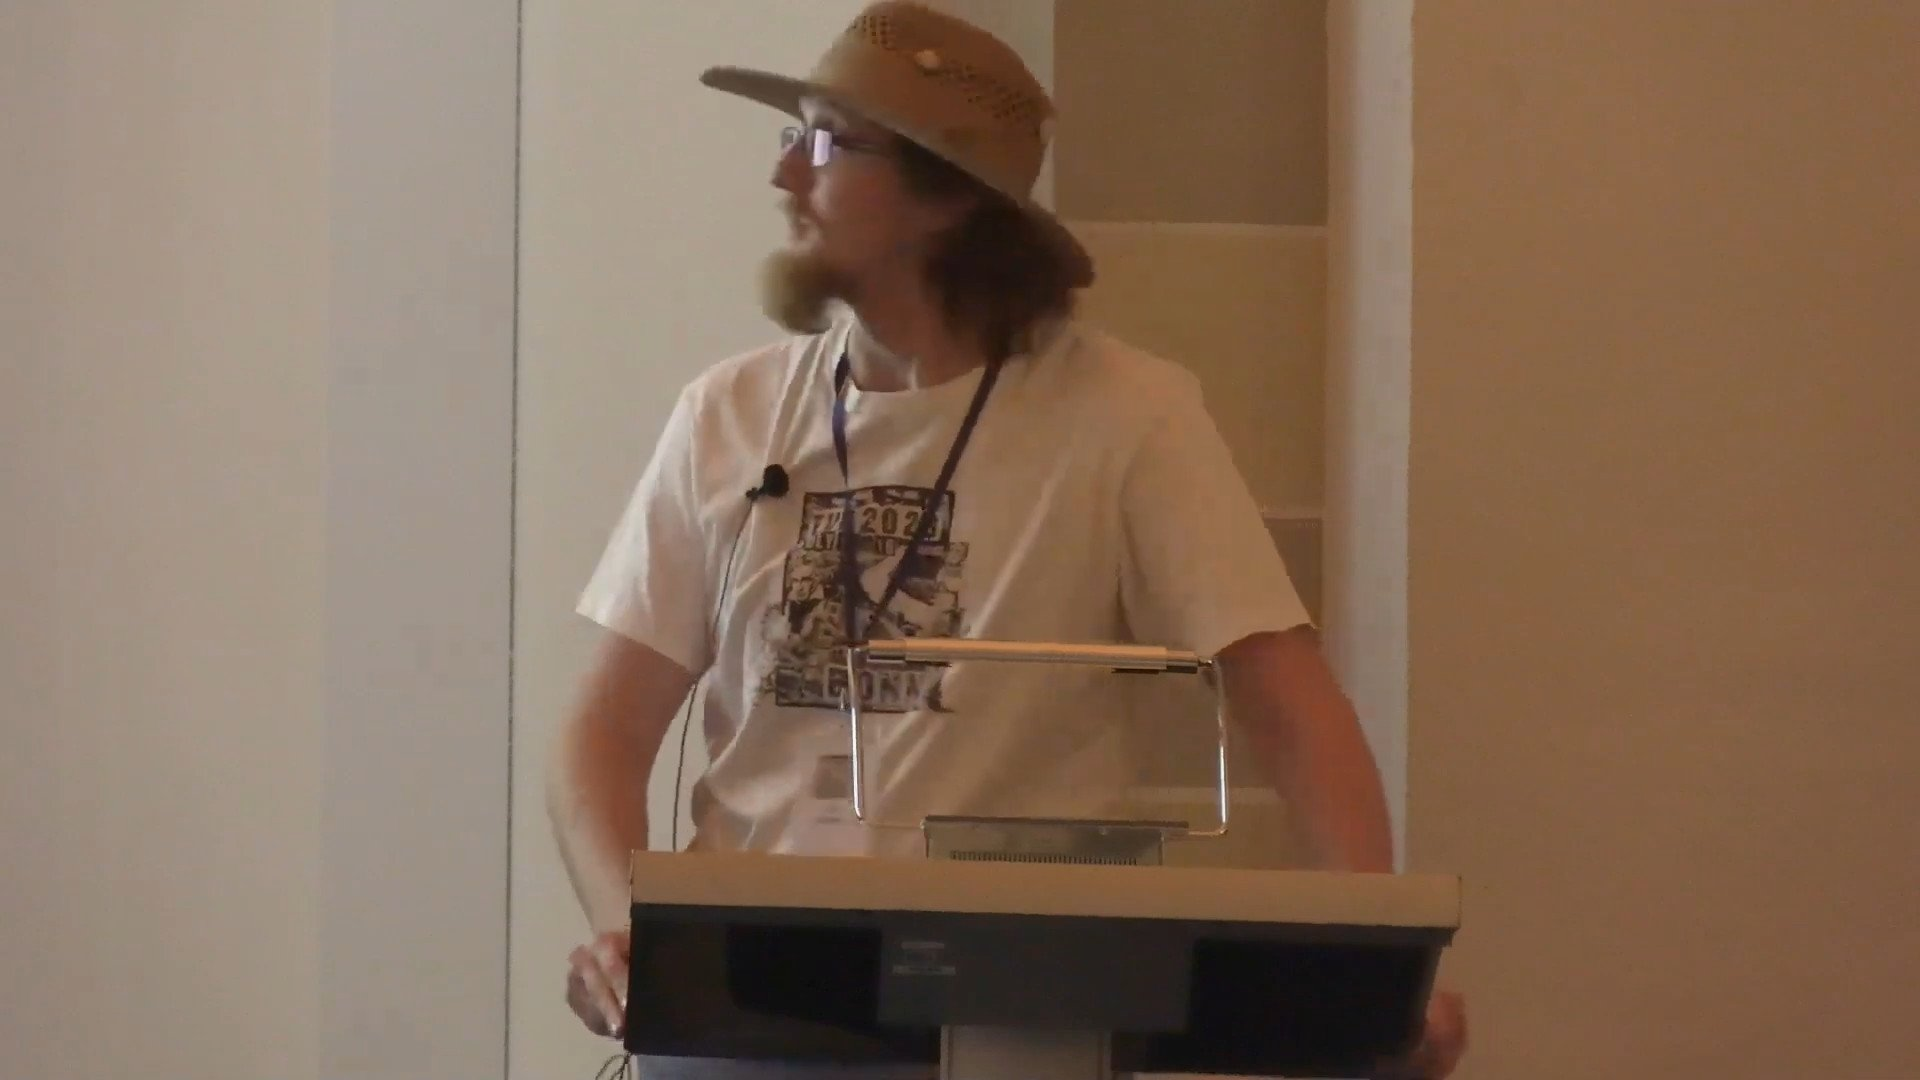
\includegraphics[width=0.425\linewidth]{figs/talk-foreground}%
\caption*{Obrázek: Přednáškové slajdy (vlevo)~\cite{novotny2023markdowna} a videozáznam přednášky (vpravo)~\cite{novotny2023markdownb}.}
\end{figure}

\inputsubtitles[s/.$//;]{16}{17}~\cite{thompson2010pandoc},
\inputsubtitles{17}{25}

\inputsubtitles{25}{35}

\inputsubtitles{35}{42}

\inputsubtitles{42}{44}

\subsection{Motivace pro \TeX perty}

\inputsubtitles{44}{48}

\inputsubtitles{48}{52}
\inputsubtitles[s/.$//;]{52}{53}~\cite{novotny2016sazba}.
\inputsubtitles{53}{55}

\inputsubtitles{55}{60}

\inputsubtitles{60}{62}

\subsection{Motivace pro softwarové vývojáře}

\inputsubtitles{62}{67}

\inputsubtitles{67}{74}

\inputsubtitles{74}{77}
\inputsubtitles[s/.$//;]{77}{78}~\cite[sekce~2.2]{novotny2022markdownb}.

\subsection{Obsah}

\inputsubtitles{78}{88}

\inputsubtitles{88}{92}

\section{Co je nového?}

\inputsubtitles{92}{93}

\subsection{Podpora standardu CommonMark}

\inputsubtitles{93}{97}

\inputsubtitles{97}{102}

\inputsubtitles{102}{105}

\inputsubtitles{105}{107}
\inputsubtitles[s/.$//;]{107}{108}~\cite{gencur2023implementation}.
\inputsubtitles{108}{111}

\inputsubtitles{111}{115}

\subsection{Nová syntaktická rozšíření}

\inputsubtitles{115}{119}

\subsubsection{Metadata}

\inputsubtitles{119}{122}

\inputsubtitles{122}{128}

\inputsubtitles{128}{129}
\inputsubtitles[s/, které vidíte.*//;]{129}{130}~\autocites[sekce~2.1]{novotny2022markdowna}[sekce~2.1]{novotny2022markdownb}.
\inputsubtitles{130}{132}

\subsubsection{Atributy}

\inputsubtitles{132}{137}

\inputsubtitles{137}{140}
\inputsubtitles[s/.$//;]{140}{141}~\cite{novotny2023attributes}.

\subsubsection{Hybridní značkování}

\inputsubtitles{141}{146}

\inputsubtitles{146}{157}

\inputsubtitles{158}{162}
\inputsubtitles{162}{163}~\cite{novotny2023side}
\inputsubtitles{163}{165}
\inputsubtitles[s/.$//;]{165}{166}~\cite[sekce~2.3.1.38]{novotny2023markdownc}.

\subsubsection{Další syntaktická rozšíření}

\inputsubtitles{166}{170}
\inputsubtitles[s/.$//;]{170}{171}~\autocites[sekce~1]{novotny2022markdowna}[sekce~1]{novotny2022markdownb}.
\inputsubtitles{171}{173}
\oldlooseness=-1

\subsection{Nové formáty \TeX u}

\inputsubtitles{173}{176}

\inputsubtitles{176}{182}

\inputsubtitles[s/.$//;]{182}{183}~\cite{novotny2023examples}.

\subsection{Vazba na konverzní program Pandoc}

\inputsubtitles{183}{189}

\inputsubtitles{189}{190}
\inputsubtitles[s/.$//;]{190}{191}~\cite{rehak2023generic}.
\inputsubtitles{191}{196}

% Odkaz na [článek][1] a BP Dominika Reháka
%
% [1]: https://dml.cz/handle/10338.dmlcz/150298

\subsection{Dceřiné softwarové balíčky Markdownu}

\inputsubtitles{196}{200}

\inputsubtitles{200}{205}
\inputsubtitles[s/.$//;]{205}{206}~\cite{lee2023lua}.

\inputsubtitles{206}{210}
\inputsubtitles[s/.$//;]{210}{211}~\cite{novotny2022lt3luabridge}.

\subsection{Komunikace a správa projektu}

\inputsubtitles{211}{214}

\inputsubtitles{214}{216}
\inputsubtitles[s/.$//;]{216}{217}~\cite{novotny2022discord, novotny2022matrix},
\inputsubtitles{217}{220}

\section{Co se chystá?}

\inputsubtitles{220}{222}

\subsection{Stabilní verze 3.0.0}

\inputsubtitles{222}{225}%
\footnote{Verze 3.0.0 balíčku Markdown vyšla již 25. srpna 2023~\cite{novotny2023markdownd} a zahrnuje všechny opravy a změny, které popisuji v sekcích \ref{sec:otevrene-problemy} a \ref{sec:nova-syntakticka-rozsireni}.}
\inputsubtitles{225}{230}

\subsubsection{Otevřené problémy}
\label{sec:otevrene-problemy}

\inputsubtitles{230}{232}

\inputsubtitles[s/.$//;]{232}{233}~\cite{novotny2023fix}.
\inputsubtitles{233}{234}

\inputsubtitles[s/.$//;]{234}{235}~\cite{novotny2023implement},
\inputsubtitles{235}{242}

\inputsubtitles{242}{243}
\inputsubtitles[s/.$//;]{243}{244}~\cite{novotny2023make},
\inputsubtitles{244}{245}

\subsubsection{Nová syntaktická rozšíření}
\label{sec:nova-syntakticka-rozsireni}

\inputsubtitles{245}{248}

\inputsubtitles{248}{249}
\inputsubtitles[s/.$//;]{249}{250}~\cite{novotny2023adda}.
\inputsubtitles{250}{251}

\inputsubtitles[s/.$//;]{251}{252}~\cite{novotny2018add}.
\inputsubtitles{252}{263}

\subsubsection{Průvodce migrací z Markdownu 2}

\inputsubtitles{263}{266}

\inputsubtitles{266}{272}

\inputsubtitles{272}{276}

\inputsubtitles[s/2023 s/2023|,|,s/;]{276}{283}

\subsection{Budoucí rozvoj}

\inputsubtitles{283}{284}

\vspace{-0.5cm}

\subsubsection{Implicitní identifikátory sekcí}

\inputsubtitles{284}{285}
\inputsubtitles[s/.$//;]{285}{286}~\cite{novotny2022adda, novotny2022addb}.

\vspace{-0.25cm}

\subsubsection{Řízení horizontálního členění textu}

\inputsubtitles{286}{292}

\inputsubtitles[s/.$/:/;]{292}{293}
\texttt{\textbackslash markdownInput[\textsl{contentLevel = inline}]\{obsah-hlavičky-dokumentu.md\}}\\
\inputsubtitles{293}{296}
\inputsubtitles[s/.$/~|cite{novotny2023addb}:/;]{296}{297}\\
\texttt{\TeX ový odstavec s \textsl{\textbackslash markinline|[hypertextovým odkazem](http://...)|}.}

\vspace{-0.25cm}

\subsubsection{Vestavěná podpora formátu Op\TeX}

\inputsubtitles{297}{301}
\inputsubtitles[s/.$//;]{301}{302}~\cite{novotny2022support}.

\vspace{-0.25cm}

\subsubsection{Vestavěná podpora generického \TeX ového výstupu v Pandocu}

\inputsubtitles{302}{310}

\vspace{-0.25cm}

\subsubsection{Víceformátová témata}

\inputsubtitles{311}{316}

\inputsubtitles{316}{317}~\cite{novotny2021markdown}
\inputsubtitles{317}{320}
\inputsubtitles[s/.$//;]{320}{321}~\cite{novotny2023addc}.
\inputsubtitles{321}{327}

% Odkaz na [předchozí článek][1]
%
% [1]: https://dml.cz/handle/10338.dmlcz/150297

\subsubsection{Mailing list a decentralizovaná správa}

\inputsubtitles{327}{331}

\inputsubtitles{331}{336}

\section{Závěr}

\inputsubtitles{336}{341}

\inputsubtitles{341}{343}
\inputsubtitles[s/ Děkuji!/|par Děkuji!/;]{343}{344}

\section{Dotazy publika}

\begingroup
\parindent=0pt
\parskip=.5\baselineskip plus 2pt

\emph{Moderátor:} \inputsubtitles{345}{348}

\inputsubtitles{348}{350}

\emph{Moderátor:} \inputsubtitles{350}{353}

\inputsubtitles{353}{357}

\emph{Moderátor:} \inputsubtitles{357}{359}

\emph{Michael Schlüter:} \inputsubtitles{359}{376}

\inputsubtitles{376}{378}

\endgroup

\inputsubtitles{378}{385}

\inputsubtitles{385}{392}

\begingroup
\parindent=0pt
\parskip=.5\baselineskip plus 2pt

\emph{Moderátor:} \inputsubtitles{392}{393}

\emph{Henri Menke:} \inputsubtitles{393}{397}

\inputsubtitles{397}{398}

\emph{Moderátor:} \inputsubtitles{398}{399}

\emph{Posluchač:} \inputsubtitles{399}{405}

\inputsubtitles{405}{407}

\emph{Posluchač:} \inputsubtitles{407}{411}

\inputsubtitles{411}{418}

\emph{Moderátor:} \inputsubtitles{418}{419}

\emph{Barbara Beeton:} \inputsubtitles{419}{420}

\inputsubtitles{420}{421}

\inputsubtitles{421}{422}

\inputsubtitles{422}{423}

\emph{Moderátor:} \inputsubtitles{423}{424}

\inputsubtitles{424}{425}

\emph{Moderátor:} \inputsubtitles{425}{426}

\inputsubtitles{426}{427}

\endgroup

\begingroup
\sloppy
\printbibliography
\endgroup

\begin{summary}
The Markdown package for \TeX{} has provided an extensible and format-agnostic markup language for the past seven years. In this article, I present the third major release of the Markdown package and the changes it brings compared to version 2.10.0. In the article, I target the three major stakeholders of the Markdown package. Writers will learn about the new elements, which they can type in their Markdown documents, \TeX perts will learn how they can style Markdown documents in different \TeX{} formats, and developers will learn about the governance and the development of the Markdown package and how they can extend Markdown with new elements. The article is a Czech translation of my talk at TUG 2023~\cite{novotny2023markdowna, novotny2023markdownb}.

\keywords: Markdown, CommonMark, Lua, \TeX, \LaTeX, Op\TeX, Pandoc
\end{summary}
\end{document}
